\documentclass{fhnwreport} %
\usepackage[ngerman]{babel}
\usepackage[T1]{fontenc}
\usepackage[utf8x]{inputenc}
\usepackage{tikz}
\usepackage{amsmath}
\usetikzlibrary{arrows}
\usepackage{lmodern}      % Type1-Schriftart f�r nicht-englische Texte
\usepackage{float}
\usetikzlibrary{shapes}
\usetikzlibrary{intersections}
\usepackage{circuitikz}
\usepackage{transparent}

%%% Harvard-Style Bibliographie
%\usepackage{natbib}
%\bibliographystyle{agsm}

%%% IEEE-Style Bibliographie
\bibliographystyle{IEEEtran}

%% Und wenn die Bibliographie im Inhaltsverzeichnis sein soll:
\usepackage[nottoc]{tocbibind}


\title{%
  Projekt 5\\[2ex]
  Software Defined Radio}
\author{%
  Noah Hüsser und Francesco Rovelli}

\begin{document}

% Titel
\maketitle

\vfill

% Titelbild
% (kann man nat�rlich auch mit Includegraphics machen)
\begin{minipage}{\textwidth}
\begin{center}
\vspace*{5ex}
    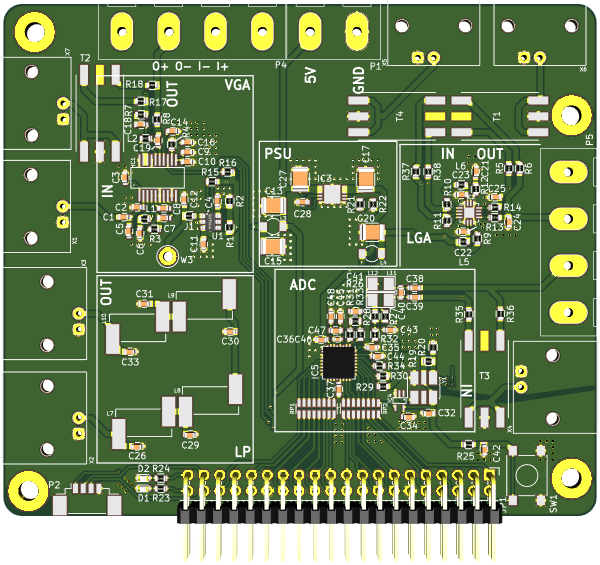
\includegraphics[height=0.4\textwidth]{data/images/title.png}
\end{center}
\end{minipage}

\vfill

\begin{tabbing}
Auftraggeber: \hspace{2em} \=  Dr. Markus Hufschmid \\[2ex]
Betreuer:  \>  Dr. Markus Hufschmid \\[2ex]
Experte:  \>  Dr. Markus Hufschmid \\[2ex]
Team:  \> Noah Hüsser \\ 
\> Francesco Rovelli \\[2ex]
Studiengang: \> Elektro- und Informationstechnik
\end{tabbing}


\hbox{}

\clearpage

\abstract{KEKEKEKEKEKEKEKEEKEK}
\clearpage

\tableofcontents
\clearpage

\section{Motivation}
\label{sec:motivation}
% FRANCESCO
Im Projekt 'Software Defined Radio mit FPGA' von Jonas Walter und Patrick Studer wurde ein SDR-Empänger auf Basis eines FPGA-Entwicklerboards aufgebaut. Dazu wurde im verlauf des Projekts ein analoges Frontend sowie Software für den FPGA entwickelt. Das Projekt war erfolgreich und konnte beim Abschluss einen funktionsfähigen Prototypen vorweisen.
Der grosse Vorteil der Auslagerung von Signalverarbeitung in den digitalen Bereich liegt in der hohen Flexibilität und dem im Vergleich kleinen Aufwand zur Funktionserweiterung.
% FREQUENZBAND-VISUALISIERUNG, blabla über frequenzbereich
Dieses Projekt versteht sich als Fortführung und möchte bestimmte Bereiche des existierenden Prototypen überarbeiten.

\clearpage

\section{Theorie}
\label{sec:sdr}
% FRANCESCO

\clearpage

\section{Ausgangslage}
\label{sec:ausgangslage}
Aus dem Vorgängerprojekt ist ein funktionsfähiger Prototyp eines SDR-Empfängers entstanden. Im Verlaufe des Projektes wurden jedoch mehrere Schwachpunkte und noch durchzuführende Arbeiten identifiziert. Viele davon entfallen auf den digitalen Teil. Die folgenden Punkte wurden zur Verbesserung im analogen Teil aufgelistet:

\begin{itemize}
	\item Anpassungen der Dimensionierung mehrerer passiver Komponenten
	\item Es fehlt ein Linearregler als rauscharme Stromversorgung
	\item Es fehlt ein Digital-Analog-Wandlers zum Einstellen der Verstärkung.
	\item Die Massenfläche sollte neu entworfen werden.
	\item Auf Signalleitungen treten Spannungsspitzen auf.
	\item Bei Frequenzen unter 2 MHz ist die Verstärkung deutlich geringer als erwartet.
	\item Die Verstärkung des einstellbaren Verstärkers entspricht nicht dem erwarteten Wert sondern hat einen Versatz
\end{itemize}


\clearpage

\section{Design des Analogen Frontends}
\label{sec:afe}
% NOAH

Die Rahmenbedingungen für das Analoge Frontend (AFE) waren durch die Vorgängerarbeit bereits gegeben. Diese sind in \ref{sec:ausgangslage} genauer erläutert.

\subsection{Schaltungsdesign}

Das AFE ist eine Kette aus Verstärkerstufen an deren Ende ein ADC das Signal abtastet. Diese Kette ist in Abbildung \ref{fig:chain} zu sehen.

\begin{figure}[H]
    \begin{center}
        \tikzset{font={\fontsize{8pt}{12}\selectfont}}
        \begin{tikzpicture}[x=0.021\linewidth,y=0.021\linewidth]

            % AD8331

            \draw[name path=lna] (0,0) node{}
            -- (0,6) node{}
            -- (6,3) node{}
            -- cycle;

            \node at (2, 3) {13dB};
            \node at (3, -1) {LNA};

            \draw[name path=attenuator] (7, 0) node{}
            -- (7, 6) node{}
            -- (13, 6) node{}
            -- (13, 0) node{}
            -- cycle;

            \draw[name path=dac] (7, 8) node{}
            -- (7, 14) node{}
            -- (13, 14) node{}
            -- (13, 8) node{}
            -- cycle;

            \draw[name path=vgain, pos=0.5, sloped, above] (10, 6) node{}
            -- (10, 8) node{$V_{GAIN}$};

            \node at (10, 11) {MCP4706};

            \draw[name path=fpga] (21, 8) node{}
            -- (21, 14) node{}
            -- (42, 14) node{}
            -- (42, 8) node{}
            -- cycle;

            \node at (31.5, 11) {FPGA};

            \draw[name path=hilo, pos=0.5, sloped, above] (24, 4.5) node{}
            -- (24, 8) node{HILO};

            \draw[name path=i2c, pos=0.5, sloped, above left] (13, 11) node{}
            -- (21, 11) node{$I^2C$};

            \draw[name path=parallel] (39, 6) node{}
            -- (39, 8) node{};

            \node at (10, 3) {0 to 40 dB};
            \node at (10, -1) {Attenuator};

            \draw[name path=fga] (14,0) node{}
            -- (14,6) node{}
            -- (20,3) node{}
            -- cycle;

            \node at (16, 3) {21dB};
            \node at (17, -1) {FGA};

            \draw[name path=vga] (21,0) node{}
            -- (21,6) node{}
            -- (27,3) node{}
            -- cycle;

            \node[align=left] at (23, 3) {3.5dB \\ 15.5dB};
            \node at (24, -1) {VGA};

            \draw[name path=AD8331] (-0.5, -2) node{}
            -- (-0.5, 7) node{}
            -- (27.5, 7) node{}
            -- (27.5, -2) node{}
            -- cycle;

            \node at (1.5, -3) {AD8331};

            % ISL55210

            \draw[name path=pa] (28.5,0) node{}
            -- (28.5,6) node{}
            -- (34.5,3) node{}
            -- cycle;

            \node at (30.5, 3) {28.5dB};
            \node at (31.5, -1) {PA};

            \draw[name path=ISL55210] (28, -2) node{}
            -- (28, 7) node{}
            -- (35, 7) node{}
            -- (35, -2) node{}
            -- cycle;

            \node at (30, -3) {ISL55210};

            % LTC2252

            \draw[name path=adc] (36, 0) node{}
            -- (36, 6) node{}
            -- (42, 6) node{}
            -- (42, 0) node{}
            -- cycle;

            \node[align=center] at (39, 3) {12 bit \\ 105 $\frac{MS}{s}$};
            \node at (39, -1) {ADC};

            \draw[name path=LTC2252] (35.5, -2) node{}
            -- (35.5, 7) node{}
            -- (42.5, 7) node{}
            -- (42.5, -2) node{}
            -- cycle;

            \node at (37.5, -3) {LTC2252};

            \path[name path=lineA] (0, 2) coordinate (A1) node{}
            -- (41, 2) coordinate (A2) node{};

            \path[name path=lineB] (0, 4) coordinate (B1) node{}
            -- (41, 4) coordinate (B2) node{};

            \path [name intersections={of=lineA and lna, name=CS1}];
            \path [name intersections={of=lineA and attenuator, name=CS2}];
            \draw[] (CS1-2) -- (CS2-1);
            \path [name intersections={of=lineA and fga, name=CS3}];
            \draw[] (CS2-2) -- (CS3-1);
            \path [name intersections={of=lineA and vga, name=CS4}];
            \draw[] (CS3-2) -- (CS4-1);
            \path [name intersections={of=lineA and pa, name=CS5}];
            \draw[] (CS4-2) -- (CS5-1);
            \path [name intersections={of=lineA and adc, name=CS6}];
            \draw[] (CS5-2) -- (CS6-1);

            \path [name intersections={of=lineB and lna, name=CS1}];
            \path [name intersections={of=lineB and attenuator, name=CS2}];
            \draw[] (CS1-2) -- (CS2-1);
            \path [name intersections={of=lineB and fga, name=CS3}];
            \draw[] (CS2-2) -- (CS3-1);
            \path [name intersections={of=lineB and vga, name=CS4}];
            \draw[] (CS3-2) -- (CS4-1);
            \path [name intersections={of=lineB and pa, name=CS5}];
            \draw[] (CS4-2) -- (CS5-1);
            \path [name intersections={of=lineB and adc, name=CS6}];
            \draw[] (CS5-2) -- (CS6-1);
        \end{tikzpicture}
    \end{center}
    \caption{Blockschaltbild des Analogen Frontends}
    \label{fig:chain}
\end{figure}

Diese Anordnung wurde so im Vorgängerprojekt gewählt um eine gewünschte verstellbare Verstärkung von 24 - 84 dB zu erhalten.
Da aber nicht alles so reibungslos funktionierte wie gewünscht, wurden alle Komponenten noch einmal sogrfältig durchgegangen und eine Leiterplatte gefertigt, welche die Komponenten einzeln aufbaut und die Möglichkeit hat diese so separat auszumessen.

Ausser dem DAC und dem Spannungswandler von 5 auf 3.3 Volt war im Vorgängerprojekt alle aktiven Komponenten gleich vorhanden. Diese Komponenten wurden aufgrund der früher (Kapitel \ref{sec:ausgangslage}) genannten Mängel gewählt und implementiert.

\subsubsection{AD8331}

Der AD8331\cite{AD8331} ist ein Vorverstärker, der fixe Verstärkerstufen im Innern hat und dazu ein Dämpfungsglied, welches so eine verstellbare Verstärkung ermöglicht. Ausserdem kann wahlweise eine von zwei vorgegebenen Verstärkungen zugeschaltet werden. Dieser Aufbau ist in Grafik \ref{fig:AD8331} dargestellt.

\begin{figure}[H]
\begin{center}
    \includegraphics[trim={11.5cm 18.3cm .5cm 5cm},clip,scale=1.5]{../AD8331_8332_8334_Datasheet}
    \caption{A8331 Blockschaltbild aus dem Datenblatt\cite{AD8331}.}
    \label{fig:AD8331}
\end{center}
\end{figure}

Der erste Verstärker erwartet ein asymmetrisches Signal, auch single-ended genannt, am Eingang und verstärkt es um 19 dB, versieht es mit einem Bias und gibt ein differentielles Signal zurück. Nach dieser Stufe sind alle Signale differentiell.
Diese Stufe muss dann extern zum Dämpfungsglied geschaltet werden. Es wäre gut möglich hier noch extern ein Filter zuzuschalten. In dieser Anwendung wurden einfach 100n Kondensatoren dazwischen geschaltet um noch einmal DC zu blocken. % TODO überarbeiten
Die Dämpfung des Dämpfungsgliedes ist stufenlos von 0 bis 48 dB übder den GAIN-Pin verstellbar. Hierfür wurde ein einfacher DAC verwendet. Dazu in Abschnitt \ref{subsec:MCP4706} mehr.
Zuletzt wird ein Nachverstärker zugeschaltet der noch einmal 3.5 oder 15.5 dB verstärkt. Die Verstärkung kann über den HILO-Pin gewählt werden.
Ausserdem kann die Ausgangsspannung auf ein Maximum begrenzt werden, was nützlich ist um weitere Bauteile vor Überspannung zu schützen.

Die totale Verstärkung kann einfach mit den Formeln\cite{AD8331} in \ref{eq:A8331_LO} und \ref{eq:A8331_HI} erhalten werden.

\begin{equation}
    G_{dB} = 50 \frac{dB}{V} \cdot V_{GAIN} - 6.5 dB, HILO = LO
\label{eq:A8331_LO}
\end{equation}

\begin{equation}
    G_{dB} = 50 \frac{dB}{V} \cdot V_{GAIN} - 6.5 dB, HILO = HI
\label{eq:A8331_HI}
\end{equation}

\subsubsection{ISL55210}
Der ISL55210\cite{ISL55210} ist ein differentieller Verstärker. Er wird normal mit Feedbackwiderständen beschaltet\cite{ImpedanceMatching2009}, so dass die gewünschte Verstärkung von 28.5 dB erreicht wird.
Er hat ein GBWP von 4 Ghz was für das geplante SDR alleweil reicht, da nur Signale bis 30 Mhz von Interesse sind. Bei einer Verstärkung von 28.5 dB ist das GBWP also noch lange nicht ausgereizt.

\subsubsection{LTC2252}
Es wurde der LTC2252\cite{LTC2252} mit 12 Bit als A/D-Wandler gewählt. Erfahrungen aus dem Vorgängerprojekt haben gezeigt, dass höhere Auflösungen nicht einfach zu einem besseren Resultat führen. % TODO Hufi's Argumentation .
Mit 105 MS/s ist er sicher genug schnell um Aliasing zu verhinden, wenn man annimmt dass bei einer Cutoffrequenz von 30 MHz das Eingangsfilter 9. Ordnung bei 50 Mhz um etwa 50dB gedämpft wird.
Die Beschaltung wurde aus dem Application Note übernommen. Hier wurde viel Augenmerk darauf gelegt die Anweisungen im Application Note akribisch zu befolgen. Dies war dann insbesondere im Leiterplattendesign wichtig, was im Abschnitt \ref{subsec:Leiterplattendesign} genauer besprochen wird.

\subsubsection{MCP4706}
\label{subsec:MCP4706}
Der MCP4706\cite{MCP4706} ist ein 8 bit Digital-Analog-Konverter. Er wird dazu genutzt die variable Verstärkung des AD8331 mittels einer Spannung einzustellen. Er wurde so konfiguriert dass er maximal ein Volt Ausgangsspannung hat, da dies die Grenze für den AD8331 ist. Gleichzeitig gehen zehn Skalierungsstufen verloren, da der AD8331 als Untergrenze 40 mV erwartet. Somit geht der zulässige Wertebereich für den DAC von 11 bis 255, was genügend dynamic Range sein sollte. Wieviel Verstärkung das Erhöhen des Wertes am DAC um eins zum Ergebnis hat sieht man in Gleichung \ref{eq:DAC_wert}.

\begin{equation}
    \Delta G_{dB} = 50 \frac{dB}{V} \cdot \frac{1}{2^8 - 1} = 0.196 dB
\label{eq:DAC_wert}
\end{equation}

Der DAC ist über $I^2 C$ bequem ansteuerbar. Dies war eine wichtiges Auswahlkriterium zusammen mit einem rauscharmen Ausgang. Der MCP4706 hat eine simple Resistorladder, das heisst, es werden je nach Ausgangswert Widerstände dazu- oder weggeschaltet. Damit sollte die Spannung am DAC-Ausgang praktisch keine Schwankungen erfahren, beziehungsweise ist es nur vom Rauschen der Spannungsversorgung abhängig, wie in \ref{eq:DAC_rauschen2} ersichtlich ist. Nimmt man an, dass $\Delta f \xrightarrow 0$, da die Verstärkung einmal zu beginn der Übermittlung eingestellt wird und dann statisch bleibt, so sieht man dass das Rauschen vernachlässigbar wird.

\begin{equation}
    U_N = \sqrt{4 \cdot k_B \cdot T \cdot \Delta f \cdot R},\,k_B = 1.38\cdot 10^{-23}\frac{J}{K},\,T = 300K,\,R = 210k\Omega
\label{eq:DAC_rauschen}
\end{equation}

\begin{equation}
    U_N = \sqrt{4.1751\cdot 10^{-15} \cdot \Delta f}
\label{eq:DAC_rauschen2}
\end{equation}

\subsubsection{LP38798}
Der LP38798 ist ein linearer Spannungsregler mit guter Rauschdämpfung und aktivem Rippelausgleich. Er wurde anstelle eines Schaltreglers eingesetzt, da Schaltregler aufgrund ihres Funktionsprinzips tendenziell Störsignale einbringen statt, wie im Falle von Linearregler, sie zu dämpfen.
Dieser Regler im Speziellen ist auf tiefes Rauschen (5µV RMS) und einen hohen Versorgungsspannungsdurchgriff (PSRR) optimiert, weswegen er uns bei der Recherche ins Auge gestochen ist. Dies ist zur stabilen Stromversorgung der Verstärker auch bei Betrieb an einer weniger als optimalen Stromquelle von Bedeutung.
Weitere Kenndaten wie Chipgrösse, Preis und Effizienz waren bei der Auswahl von sekundärer Wichtigkeit da der Einsatz im Rahmen des Projekts auf Prototypen zur stationären Verwendung beschränkt ist.

\begin{figure}[H]
	\begin{subfigure}[b]{0.5\textwidth}
		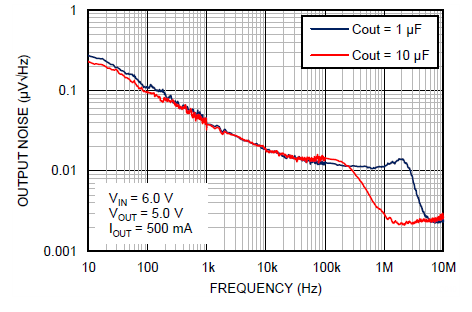
\includegraphics[clip,scale=0.6]{data/images/ldo_noise}
		\caption{Rauschen aus Datenblatt\cite{LP38798}.}
		\label{fig:ldo_rauschen}
	\end{subfigure}
	\hfill
	\begin{subfigure}[b]{0.5\textwidth}
		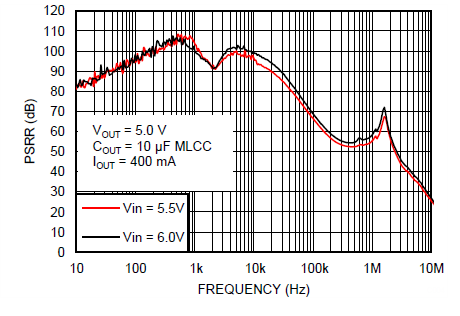
\includegraphics[clip,scale=0.6]{data/images/ldo_psrr}
		\caption{PSRR aus Datenblatt\cite{LP38798}.}
		\label{fig:ldo_psrr}
	\end{subfigure}
\end{figure}

Um Verbrauchsspitzen abzufangen wurde dem Regler ein Tiefpassfilter mit Kapazitäten nachgeschaltet.
Eine Umsetzung mit Schaltregler wäre prinzipiell vorstellbar. Eine solche Lösung hätte aber aufgrund der fehlenden architekturgegebenen Filterung zusätzliche externe Filter, speziell für die Schaltfrequenz aber auch als Ersatz des intrinsischen Filtereffekts, erfordert.

Beim Design der Leiterplatte wurde darauf geachtet, dass die leistungsführenden Leitungen bis an die Chipanschlüsse möglichst breit gehalten wurden. Zudem ist die Massenfläche zur besseren Abführung der abfallenden thermischen Leistung mehrfach durchkontaktiert.

Zur Kompensation der abnehmenden PSRR in höheren Frequenzen und Filterung der Spannung von externen Quellen ist in beiden Spannungsnetzen ein Pi-Tiefpass-Filter eingebaut.

\begin{figure}[H]
	\begin{center}
		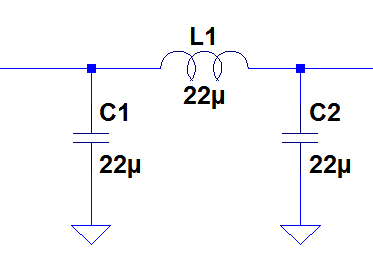
\includegraphics[clip,scale=0.4]{data/images/powerfilter}
		\caption{Schema des Rauschfilters}
		\label{fig:powerfilter}
	\end{center}
\end{figure}

% GRAFIK SIMPLOT

\subsection{Stromversorgung}
Die beiden Spannungsnetze werden wie folgt verwendet.

5V Spannungseingang, extern gespiesen:

\begin{itemize}  
	\item AD8331 (LNA / VGA)
	\item MCP4706 (DAC)
\end{itemize}

3.3V Spannungseingang, gespiesen vom Linearregler (LP38798):

\begin{itemize}  
	\item ISL55210 (Differentieller Verstärker)
	\item LTC2252 (ADC)
\end{itemize}

\clearpage
\subsection{Leiterplattendesign}
\label{subsec:Leiterplattendesign}
Die Leiterplatte wurde so ausgelegt, dass alle Komponenten (VGA, LNA, ADC) des Frontends mehr oder weniger abgekapselt auf einem Board sind. Jede Komponente kann zu der weiterführenden benachbarten geschaltet werden. Wenn die Komponenten nicht gechaint werden, so können sie am Input und am Output an einen Balun angeschlossen werden. So können alle Komponenten einzeln gemessen werden. Die Baluns sind notwendig damit die differentiellen Komponenten korrekt terminiert werden und das Signal in ein single-ended Signal umgewandelt wird. Diese zweite Eigenschaft ist voraussetzung um einen VNA anschliessen zu können.

Wichtige Änderungen zum Vorgängerprojekt bestehen hier vor allem darin, dass die Groundplane optimiert wurde und die Komponenten näher zum jeweiligen Chip angeordnet wurden.

\subsubsection*{Groundplane}
Es ist wichtig dass in einer HF-Anwendung eine möglichst unbeschädigte Groundplane vorliegt. Zum einen braucht es ein fixes Referenzpotential welches sich möglichst nicht verschieben soll. Bei mehr Masse ist das einfacher, da die Ströme keine langen Wege nehmen müssen.

\subsubsection*{Leiterbahnen}
Leiterbahnen sollten so kurz wie möglich gehalten werden. Zudem sollten symmetrische Signale auch physikalisch so gehalten werden, wenn sie über längere Distanzen geführt werden. Das heisst sie sollten geometrisch nahe beieinander gehalten und symmetrisch geroutet werden. 

\subsubsection*{AD8331}
Im Datasheet zum AD8331 gibt es einige Tipps wie das Layouten gelingt. So soll Dead Copper vermieden werden und stattdessen mit Ground verbunden werden.
Die externen Komponenten an den Pins LON und LOP sowie an den Pins VOL und VOH sollten so nahe wie möglich am Chip platziert werden um Lodading-Effekte zu vermeiden.
Zudem sollten speziell die Verbindungen von LON und LOP zu VIN und VIP möglichst kurz gehalten werden um ungewünschte Effekte zu vermeiden. Dazwischen hat es einen externen Coupling-Kondensator, da danach das Signal mit einem Bias versehen wird um es in ein differentielles Signal zu erhalten.

\subsubsection*{ISL55210}
Beim ISL55210 wurden lediglich die üblichen wichtigen Design-Richtlinien befolgt. 

\subsubsection*{LTC2252}
Der ADC ist am heikelsten zu layouten. Er hat digitale sowie analoge Komponenten. Diese müssen strikt getrennt werden, um zu vermeiden, dass digitale Signale welche viel Strom brauchen die Referenzlevel für den analogen Teil verfälschen. Es sollen Querströme vermieden werden!
Hier war schon beim Vorgängerprojekt eine Diskussion, wie das Groundlayout auszusehen hat. Dazu gibt es verschiedene Artikel insbesondere einen Artikel von Analog Devices \cite{StayingWellGrounded2012} und natürlich das Datasheet des LTC2252\cite{LTC2252} welche Hinweise geben, wie das Layout zu gestalten sei. Es gibt verschiedene Ansätze wie man vorgehen sollte. Manche bevorzugen zwei komplett getrennte Groundplanes welche an einem Punkt zusammengeführt werden und manche bevorzugen es die Groundplane als ein Ganzes zu behalten. Sie sind sich alle in einem Punkt einig: Oftmals wird falsch verstanden zu welchem Ground bzw zu welcher Versorgung ein Pin der mit DGND (digital Ground) angeschrieben ist nun gehört. So gehört dieser Pin nicht an ein digitales Referenzpotential, sondern an ein analoges! Wieso dem genau so ist, ist wunderbar erklärt in \cite{StayingWellGrounded2012}, wird hier aber nicht noch einmal aufgeführt.
Es ist unter jeden Umständen zu vermeiden den DGND des ADCs an einen digitalen Ground zu hängen! Des weiteren ist die Verbindung zwischen AGND und DGND möglichst kurz zu halten um weitere parasitäre Effekte zu vermeiden.
Es wird im Datasheet explizit erwähnt dass der Ground unter und um den Chip aus einer ungestörten Plane besteht. Es sind eher 4-Layer+ empfohlen. Es wurde bei diesem Projekt versucht so gut wie möglich mit 2 Layern auszukommen.

Im LTC2252 Datasheet wird zudem erwähnt, dass digitale und analoge Signale gut getrennt werden müssen. Diese sollten sich unter keinen Umständen in die Quere kommen um parasitäre Koplungseffekte zu vermeiden. Dies macht einem der LTC2252 zum Glück sehr leicht, da die Signale im Pinout schon sinnvoll getrennt angeordnet sind.
Die Groundplane wurde hier so eingeschnitten, dass digitale Signale nicht über den analogen Bereich zurücklaufen. Dies ist in Grafik \ref{fig:groundplane_bsp} sehr schön zu sehen.

\begin{figure}[H]
\begin{center}
    \tikzset{font={\fontsize{48pt}{12}\selectfont}}
    \begin{tikzpicture}
        \node[opacity=1]{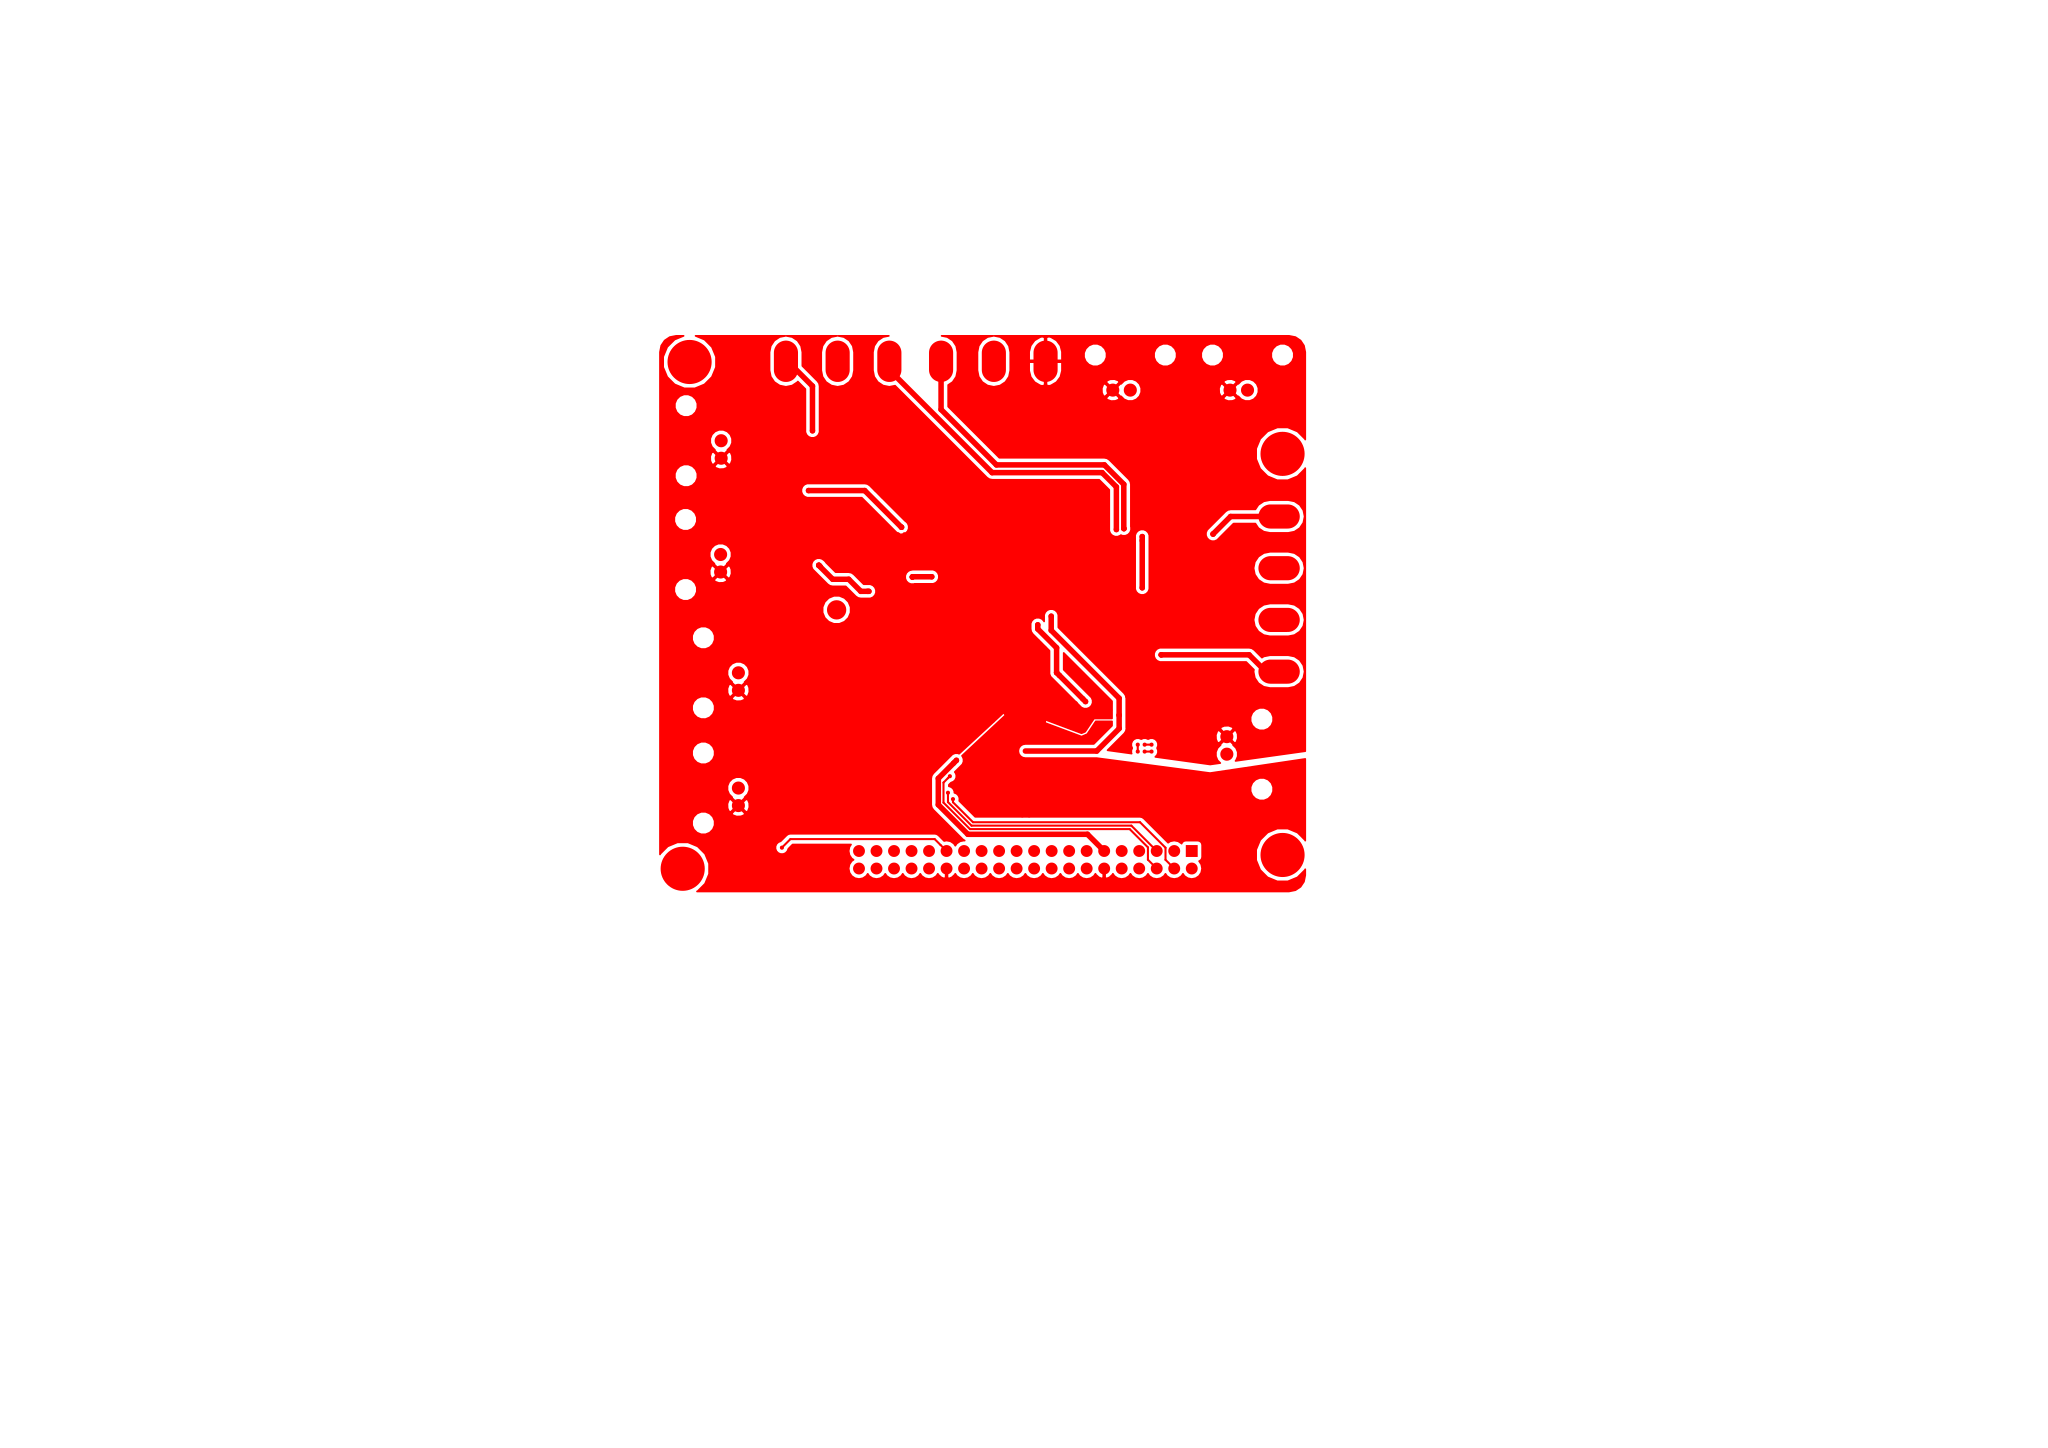
\includegraphics[trim={14cm 9.3cm 13.7cm 9.7cm},clip,scale=6]{data/images/amplifier-B_Cu}};
        \node[opacity=0.2]{\includegraphics[trim={14cm 9.3cm 13.7cm 9.7cm},clip,scale=6]{data/images/amplifier-F_Cu}};

        % Analog Area

        \draw[name path=attenuator, fill=, opacity=0.3] (-5.8, -0.5) node{}
        -- (-5.8, 5.8) node{}
        -- (5.8, 5.8) node{}
        -- (5.8, 1.8) node{}
        -- (5, 1.8) node{}
        -- (4.5, 1) node{}
        -- (4.0, 0.6) node{}
        -- (0.5, 2.3) node{}
        -- (-2.7, 2.3) node{}
        -- cycle;

        \node at (0, 4) {Analog};

        % Digital Area

        \draw[name path=attenuator, fill=, opacity=0.3] (-5.8, -1.3) node{}
        -- (-5.8, -5.8) node{}
        -- (5.8, -5.8) node{}
        -- (5.8, 1.3) node{}
        -- (5.4, 1.3) node{}
        -- (4.7, 0.2) node{}
        -- (4.2, 0) node{}
        -- (0, 1.5) node{}
        -- (-2.7, 1.5) node{}
        -- cycle;

        \node at (0, -3) {Digital};

        % ADC

        \draw[name path=attenuator] (-2, 2.2) node{}
            -- (0.5, 2.2) node{}
            -- (0.5, -0.3) node{}
            -- (-2, -0.3) node{}
            -- cycle;

        \tikzset{font={\fontsize{48pt}{12}\selectfont}}
        \node at (-0.75, 0.95) {\huge ADC};

        % DAC

        \draw[name path=attenuator] (5.8, -1.5) node{}
            -- (5, -1.5) node{}
            -- (5, -5) node{}
            -- (5.8, -5) node{};

        \node at (5, -3.25) {\huge DAC};
    \end{tikzpicture}
    \caption{Groundplane unter dem LTC2252.}
    \label{fig:groundplane_bsp}
\end{center}
\end{figure}

Speziell erwähnt im Datasheet wird vorallem der 100nF Kondensator zwischen REFH und REFL. Er darf sich nicht weiter als 1.5 mm vom Chip weg befinden. Er wird speziell aufgeführt und zum parallelen 2.2uF Kondensator wird gesagt dass dieser weiter weg sein kann, was annehmen lässt dass dies wirklich wichtig ist.

\clearpage

\section{Messungen}
\label{sec:messungen}
% BOTH

Hauptziel der Arbeit war es die Komponenten gut zu vermessen und ihre Leistung zu verifizieren.

\subsection{Setup \& Software}
Zum Messen wurden verschiedenste Gerätschaften verwendet. Manche wurden per Skript angesteuert zur Automatisierung der Messungen. Alle Geräte sind im Folgenden kurz erwähnt und beschrieben, da die Ansteuerung direkt mit deren Funktionsumfang zusammenhängt.

\subsubsection*{Hauptlabornetzgerät TODO: Name}
Das XXXX ist ein normales Labornetzgerät welches sich leider nicht fernsteuern lässt. Es speist bei den Versuchen lediglich das AFE mit 5V und übernimmt keine weitere Funktion. Es taugt für diese Funktion gut.

\subsubsection*{Oszilloskop Agilent TODO: name}
Das Oszilloskop ist hier um die Geschehnisse mit den Signalen zu beobachten. Für genaue Messungen der Verstärkung und Eingangsimpedanz der Schaltung wird zwar ein VNA verwendet, jedoch misst dieser immer nur einen RMS-Wert. Um genaue Signalverläufe zu beobachen und zum Beispiel zu ermitteln ob der Sinus vom Eingang am Ausgang überhaupt noch ein Sinus ist, wird das Oszilloskop verwendet. Es wird bei Bedarf per Hand bedient und wurde nicht per Skript angesteuert.

\subsubsection*{Arduino Due}
Da zur Ansteuerung des verwendeten DACs $I^2C$ verwendet wird, war eine Schnittstelle die $I^2C$ spricht unabdingbar. Statt bereits VHDL für das FPGA zu schreiben und eine weitere Baustelle anzufagen wurde ein Arduino verwendet. Es ist relativ einfach diesen dazu zu bringen $I^2C$ zu sprechen. Die Spannung des DACs kann somit vor der Messung eingestellt werden und danach kann ungestört gemessen werden, ohne dass der Bus dazwischenplappert und die Messungen verfälscht. Das ganze kann vom PC aus per UART gesteuert werden.
Leider wurde nach ersten Versuchen die Vermutung angestellt dass der DAC zusätzliches Rauschen mit sich bringt, weswegen im weiteren Verlauf der Messungen mit einem präzisen Labornetzgerät agiert wurde.

\subsubsection*{Kleine PSU TODO: Name}
Dieses Labornetzgerät kann per PC angesteuert werden. Was hier wichtig war ist das das Netzgerät Spannungen auf Milivolt genau einstellen kann.
Das Ansteuern per PC geschieht über das Netzwerk oder UART. Das Gerät wird über beide Schnittstellen mit LXI angesteuert. LXI ist ein textbasiertes Protokoll und damit menschenleserlich und einfach zu implementieren. Es wurde UART gewählt, da es per Netzwerk Probleme mit der Firewall gab. Dies ist möglich obwohl LXI eigentlich für LAN gedacht ist.

Zur Ansteuerung wurden einfache Python-Klassen geschrieben, welche die Parameter der Messgeräte lesen und setzen können. Das Python-Objekt hat dabei keinerlei Zustand. Jegliche Zustände werden auf dem Gerät selber verwaltet. Somit können auch jederzeit am Gerät selber Einstellungen vorgenommen werden und das Python-Interface kriegt diese ohne Schwierigkeiten mit und stellt diese angenehm über Variabeln zur Verfügung.

\subsubsection*{VNA TODO: Name}
Der Vector Network Analyzer (VNA) wird dazu verwendet ein Signal mit bekanntem Pegel und Frequenz in ein Zeitor (Mehrtor ist auch möglich aber in diesem Falle nicht gewünscht) zu geben und am Eingang, sowie am Ausgang zu messen wieviel von dem Signal noch übrig ist. So kann leicht das ganze System vermessen werden. Was der VNA genau macht ist hier(TODO: doc suchen kek) gut beschrieben.

Zum Glück konnte für die Messungen ein sehr gutes Gerät von HP verwendet werden. Es hat ein sehr einfaches Benutzerinterface und lässt sich zudem per PC ansteuern. Hier gibt es mehrere Varianten wie dies geschehen kann, es wurde jedoch wieder UART und LXI gewählt. Somit gab es nicht viel umzustellen um auch den VNA anzusprechen. Natürlich wurden nur Python-Schnittstellen für die Funktionen, welche auch verwendet wurden, implementiert um nicht den Zeitrahmen zu sprengen.

Das verwendete Gerät kann von 300kHz bis TODO: GHz messen und ist daher bestens geeignet. Zudem hat es eine Toleranz bis 10 VDC am Messeingang, was perfekt ist falls man bei ersten Experimenten mal einen Fehler macht. Leider hat der VNA als Untergenze -55dBm was er an Signal erzeugen kann. Deswegen wurde für Messungen mit der kompletten Verstärkerstufe ein -20dB Dämpfungsglied verwendet, welches das Signal noch einmal verkleinert. Für die Impedanzausmessung des AD8331 wurde auf das Dämpfungsglied verzichtet, da dies natürlich in komplett falschen Messresultaten endet.

\subsection{Erste Messungen}

Mit einer ersten bestückten Leiterplatte wurden daher mit dem Oszilloskop erste Messungten durchgeführt, welche eine generelle Funktionstüchtigkeit bezeugten, welche aber gar nicht zufriedenstellend war.

\begin{figure}[H]
\begin{center}
    \includegraphics[width=1\textwidth]{data/images/messungen/erste_messung}
    \caption{Erste Messungen des Gesamtsystems. Inkorrekt terminiert. Mit dem Oszilloskop gemessen.}
    \label{fig:messungen_erste}
\end{center}
\end{figure}

Diese Kurve sieht wahnsinnig unschön aus. Gerade bei den Peaks gibt es fiese Ausreisser. Und was ebenfalls nicht zu vernachlässigen ist, sind die 180 Grad Phasenverschiebung.
Auch sieht man hier, dass der dass der Input des Funktionsgenerators ziemlich viel Rauschen hat, welches sich auch in Grafik \ref{fig:messungen_zweite} zeigt.
Dort sieht man gut, dass der Input ziemlich rauscht. Deswegen haben wir versucht N und P voneinander zu subtrahieren. Und so das Rauschen zu eliminieren. Dies hat sogar relativ gut geklappt. Dies ist natürlich nicht ganz sauber, ging aber für eine erste Verifikation sehr gut.

\begin{figure}[H]
\begin{center}
    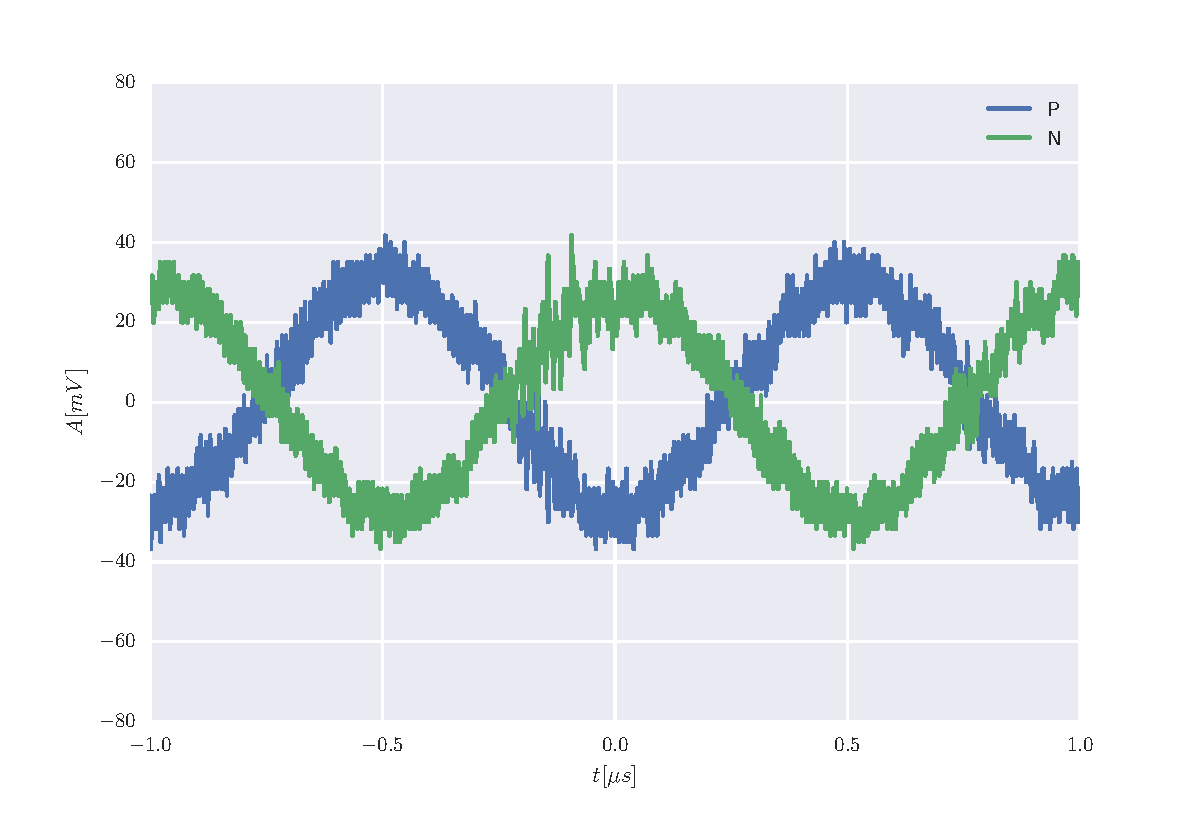
\includegraphics[width=1\textwidth]{data/images/messungen/zweite_messung_NP}
    \includegraphics[width=1\textwidth]{data/images/messungen/zweite_messung_INOUT}
    \caption{Erste Messungen des Gesamtsystems. Inkorrekt terminiert. Mit Oszilloskop gemessen.}
    \label{fig:messungen_zweite}
\end{center}
\end{figure}

Bei diesen Messungen war jedoch das DUT nicht korrekt terminiert. Dies war einer der Knackpunkte zum Anfang. Es war uns bekannt, dass Dinge in diesem Gebiet korrekt terminiert werden müssen. Wenn das DUT nicht korrekt belastet wird können ungewollte Effekte auftreten. Deswegen sind diese ersten Messungen mit Vorsicht zu geniessen und dürfen nur als Anhaltspunkt und nicht als exakte Messung genommen werden.

Eigentlich wären zur korrekten Terminierung und Umwandlung in ein single-ended Signal, wie im Abschnitt \ref{subsec:Leiterplattendesign} beschrieben, Baluns vorgesehen. Diese sind jedoch relativ schwer zu kriegen und sind dann relativ teuer. Deswegen wurde eine günstigere Lösung gesucht. Diese wurde in der in \ref{fig:terminator} dargestellten Schaltung gefunden.

\begin{figure}[H]
\begin{center}
    \begin{circuitikz}
        \draw[dotted] (-1, 0) 
        node[rground, rotate=-90]{}
        to[V,v=$U_q$, *-] (-1,2)
        to[short] (1,2);

        \draw (1,2)
        node[ocirc]{}
        to[short] (2,2)
        to[R=$222\Omega$] (4,2)
        to[short] (6, 2)
        node[ocirc]{};

        \draw (5,2)
        to[R,l_=$65\Omega$, *-*] (5,0)
        node[rground, rotate=-90]{};

        \draw[dotted] (6, 2)
        to[short] (7, 2)
        to[R=$50\Omega$] (9,2)
        to[short] (9, 0)
        node[rground]{};

        % Lower side

        \draw[dotted] (-1, 0)
        to [V,v_=$U_q$] (-1,-2)
        to[short] (1,-2);

        \draw (1,-2)
        node[ocirc]{}
        to[short] (2,-2)
        to[R=$250\Omega$] (4,-2)
        to[short] (5, -2)
        to[short] (5, 0);

        % Boxes

        \draw[dashed] (-2, 4)
        to[short] (1, 4)
        to[short] (1, -4)
        to[short] (-2, -4);

        \draw (-1, -3) node{DUT};
        \draw[->] (-1, 3) -- (0.5, 3) node [pos=0.66,above,align=center]{$250\Omega$};

        \draw[dashed] (10, 4)
        to[short] (6, 4)
        to[short] (6, -4)
        to[short] (10, -4);

        \draw (9, -3) node{VNA};
        \draw[->] (9, 3) -- (7.5, 3) node [pos=0.66,above,align=center]{$50\Omega$};

    \end{circuitikz}
    \caption{Terminierung des AD8331 zur Messung mit single-ended Geräten die 50 $\Omega$-Terminierung haben.}
    \label{fig:terminator}
\end{center}
\end{figure}

Damit sieht der AD8331 die gewünschten 250 $\Omega$ auf beiden Ausgängen des differentiellen Signales. Zugleich sieht der VNA dabei seine gewünschten 50 $\Omega$.
Diese Lösung eliminiert profitiert zwar nicht von der Störungseliminierung eines differentiellen Signales, ist jedeoch für den Rahmen dieses Projektes mehr als ausreichend.

Was jetzt noch beachtet werden muss ist der Spannungsteiler der durch diese Schaltung am Ausgang vorgeschaltet wird.
So müssen Messresultate jeweils mit $\frac{1}{a}$ multipliziert werden wobei $a$ in Gleichung \ref{eq:a_AD8331} gegeben ist.

\begin{equation}
    a = \frac{R_L}{R_S + \sqrt{R_S(R_S - 2R_L)})} = 0.1127, R_L =50, R_S = 250
    \label{eq:a_AD8331}
\end{equation}

Dieser Wert hat noch einen kleinen Fehler, da Widerstände nur endlich genau sind. In der Fehlerrechnung \ref{eq:fehler_a_AD8331} wurde ein Fehler von ±1 für $R_S$ und $R_L$ angenommen. Dies ergibt einen Relativen Fehler von 1.86\% was akzeptabel erscheint.

\begin{equation}
    \Delta a = \frac{R_s - R_L}{-2R_S\sqrt{R_S(R_S - 2R_L)}} = 0.0021, R_L = 50±1, R_S = 250±1
    \label{eq:fehler_a_AD8331}
\end{equation}

Mit korrekter Korrektur des gemessenen Wertes wurde nun je eine kleine Messreihe durchgeführt. Diese ist in Grafik \ref{fig:kaputtes_AFE} zu sehen. Wie man hier unleicht erkennen kann gibt es einen signifikanten Unterschied je nach Terminierung.
Leider kann man hier auch erkennen dass der HI/LO Pin keinerlei Einfluss auf die Verstärkung hat. Während dies bei ersten Messungen noch funktionierte, ist dies bei diesen Messungen nicht mehr funktional. Es scheint als wäre es ein Defekt an der Hardware.

\begin{figure}[H]
\begin{center}
    \includegraphics[width=1\textwidth]{data/images/messungen/kaputtes_AFE}
    \caption{Erste Messungen des kaputten A8331.}
    \label{fig:kaputtes_AFE}
\end{center}
\end{figure}

Die ersten Messungen sind aus diesem Grunde nicht mehr zu verwenden ausser zur Verifikation genereller Funktionalität. Ein zweites PCB wurde aus diesem Grund bestückt und vermessen. Dieses hat keine erkennbaren Defekte und liefert anständige erste Ergebnisse wie in \ref{fig:ganzes_AFE} ersichtlich. Diese sind im Folgenden dokumentiert.

\begin{figure}[H]
\begin{center}
    \includegraphics[width=1\textwidth]{data/images/messungen/ganzes_AFE}
    \caption{Erste verifikation des A8331.}
    \label{fig:ganzes_AFE}
\end{center}
\end{figure}

Die Inputimpedanz des A8331 sieht gut aus wie man Grafik \ref{fig:Z_in_A8331} unschwer schliessen kann.

\begin{figure}[H]
\begin{center}
    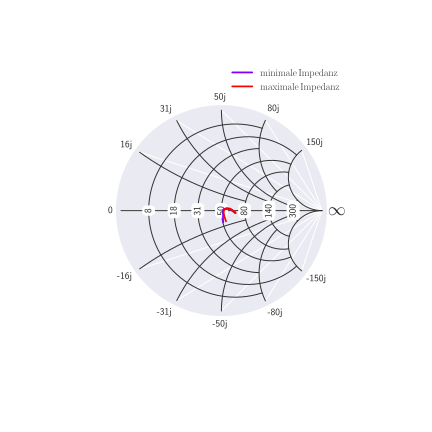
\includegraphics[width=1\textwidth]{data/images/messungen/input_Z_A8331}
    \caption{Inputimpedanz des A8331. Es sind jeweils die minimale und maximale gemessene Impedanz über alle Verstärkungen gesehen zu einer Frequenz dargestellt.}
    \label{fig:Z_in_A8331}
\end{center}
\end{figure}

Die Verstärkung sieht sehr gut aus wie Grafik \ref{fig:T_A8331} zeigt. Die Differenz zum soll ist stets kleiner als ein Dezibel. In Anbetracht des Umstandes, dass das Datasheet lediglich variable Verstärkungen auf 0.5 dB genau garantiert, ist weniger als 1 dB Abweichung extrem gut. Zudem muss berücksichtigt werden dass das Datasheet einen Verlust auf der externen Beschaltung von 0.4 dB zwischen den Pins LON und VOL sowie LOP und VOH spezifiziert.
Somit sieht die Kurve sogar noch viel besser aus.
Hier ist noch anzumerken, dass die Kurve um den Faktor $\frac{1}{a}$ und einen Faktor 2 korrigiert wurde. Der Faktor kommt daher dass das differentielle Signal nur die halbe Signalamplitude hat. 

\begin{figure}[H]
\begin{center}
    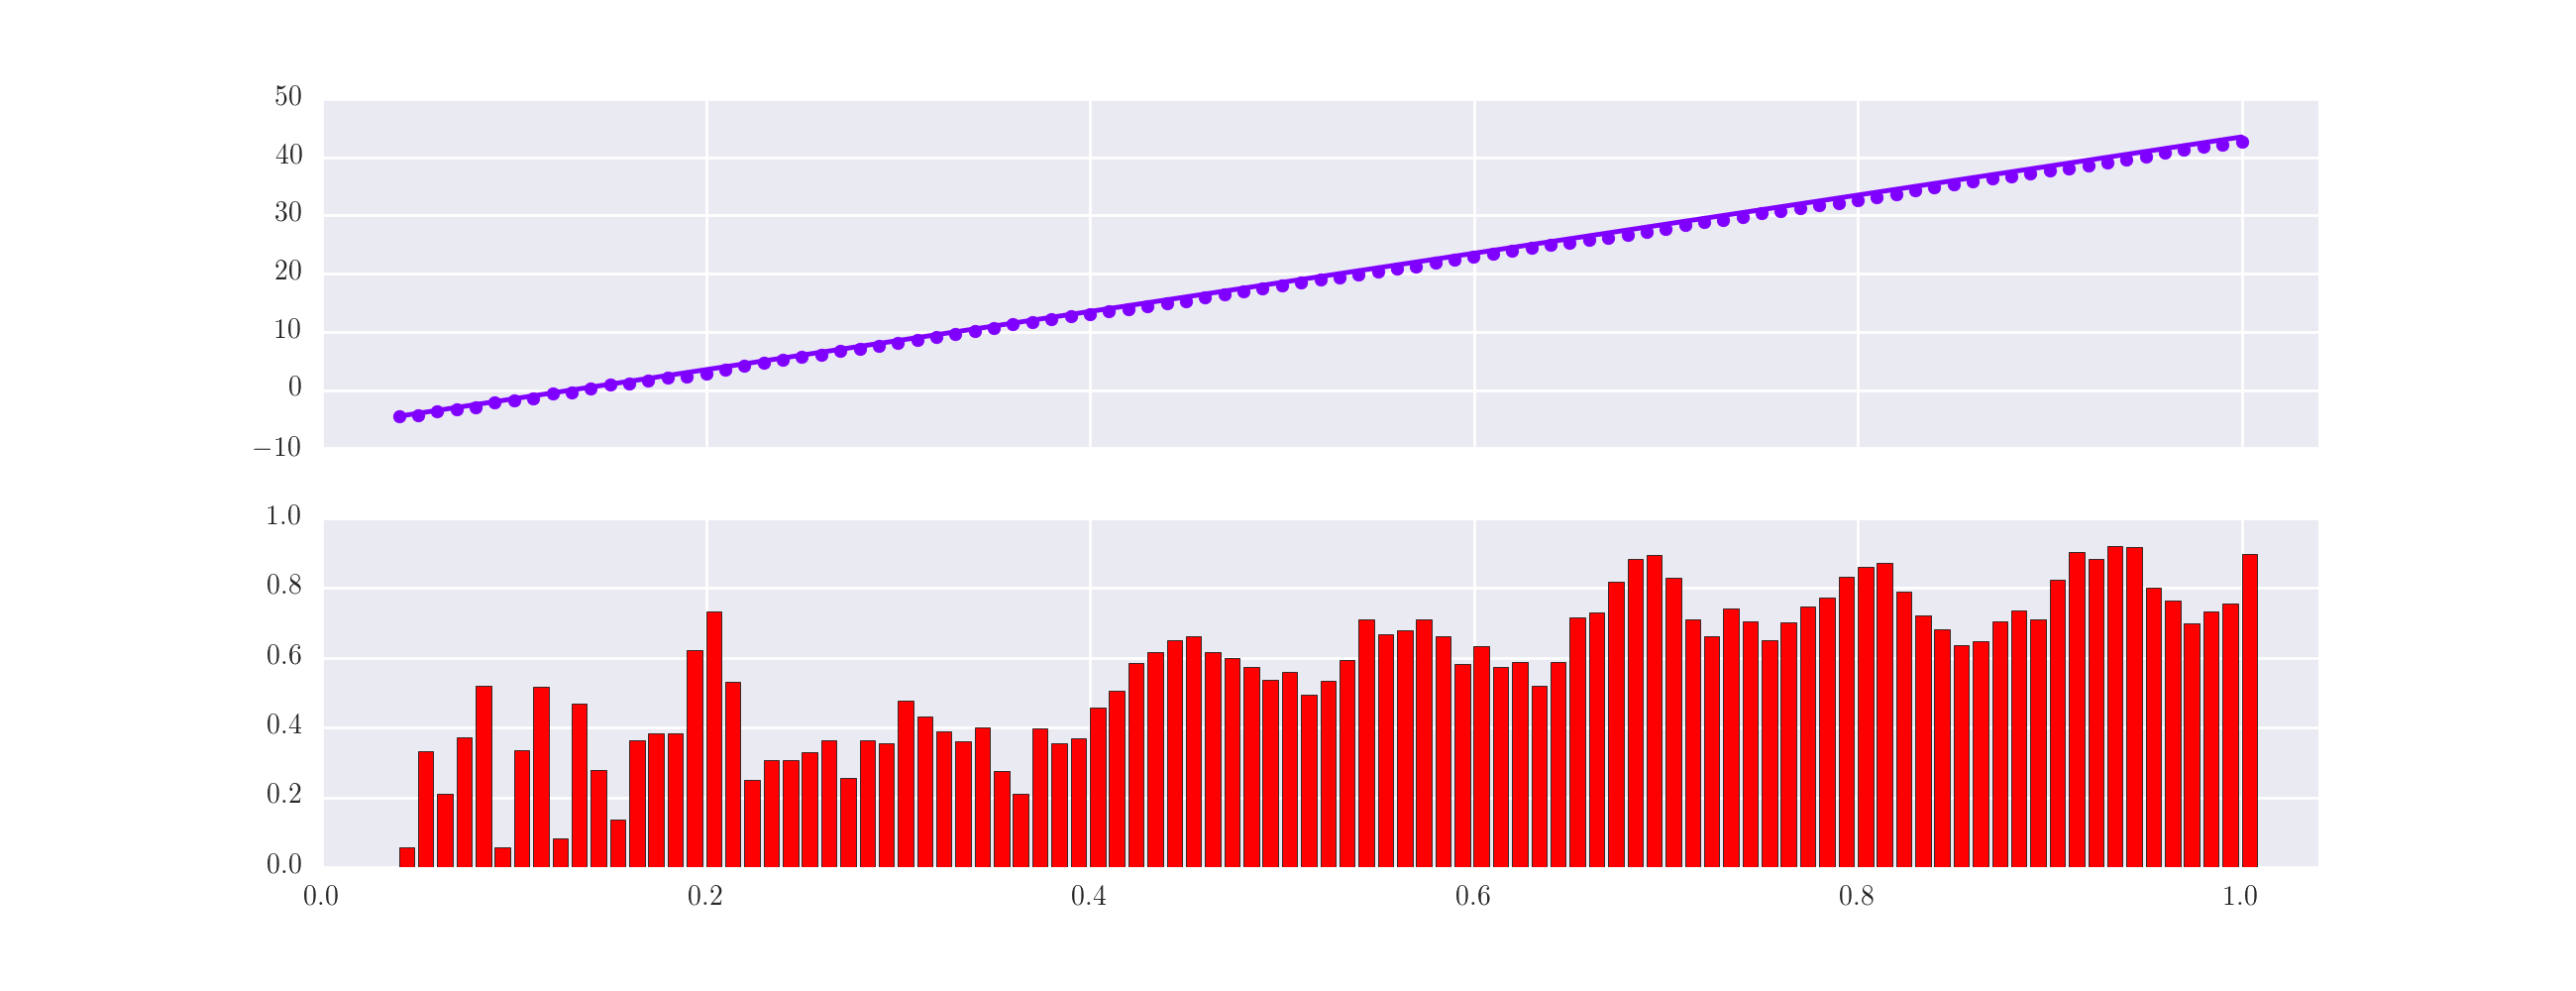
\includegraphics[width=1\textwidth]{data/images/messungen/vga_2016-12-22_30dBm_transmission2}
    \caption{Verstärkung des AD8331 gemittelt über einen 50 MHz Sweep. Ist und Soll gegenübergestellt. Zudem die Differenz zu jedem Wert.}
    \label{fig:T_A8331}
\end{center}
\end{figure}

Bei allen Messungen mit dem zweiten PCB ist der DAC nicht verbaut. Dies, da der Verdacht bestand, dass dieser viel Rauschen mit sich bringt, was nach der Erkenntniss dass der AD8331 auf dem ersten Board tatsächlich kaputt ist nicht mehr so wahrscheinlich ist. Er wurde durch eine externe Spannungsversorgung ersetzt. In weiteren Versuchen soll dieser natürlich noch genau evaluiert werden.

\subsection{ISL55210}

Da die Messungen so gut herauskamen wurde angenommen dass somit der AD8331 als Input für weitere Messungen am ISL55210 verwendet werden kann, um weiterhin auf einen Balun verzichten zu können. Mit einem twisted Pair wurden die beiden Stufen also verbunden. so kann zwar die Inputimpedanz des ISL55210 zwar nicht mehr gemessen werden, hier reichte die Transmission jedoch völlig.

Im Plot \ref{fig:T_broken_ISL55210} sieht man das Verhalten des ISL55210. Sehr unschön. Es gibt aber drei interessante Dinge zu sehen.
Erstens stimmen die gemessenen Verstärkungen über den Frequenzsweep gemittelt gut mit dem Datasheet überein wie man in Grafik \ref{fig:T_broken_mean_ISL55210} sieht.

\begin{figure}[H]
\begin{center}
    \includegraphics[width=1\textwidth]{data/images/messungen/vga_lna_2016-12-22_50dBm_20dB_transmission3}
    \caption{Verstärkung des AD8331 und ISL55210 50 MHz Sweep bei 10 verschiedenen Verstärkungen.}
    \label{fig:T_broken_ISL55210}
\end{center}
\end{figure}

\begin{figure}[H]
\begin{center}
    \includegraphics[width=1\textwidth]{data/images/messungen/vga_lna_2016-12-22_50dBm_transmission2}
    \caption{Verstärkung des AD8331 und ISL55210 gemittelt über einen 50 MHz Sweep. Ist und Soll gegenübergestellt. Zudem die Differenz zu jedem Wert.}
    \label{fig:T_broken_mean_ISL55210}
\end{center}
\end{figure}

Dies kann ein Zufall sein. Was aber viel interessanter ist, dass die Kurve zwar sehr komisch ausschaut, aber überhaupt nicht wie jene, welche beim Vorgängerprojekt gemessen wurde, wie man unschwer in Grafik \ref{fig:ganzes_system_vorganger} erkennen kann.

\begin{figure}[H]
\begin{center}
    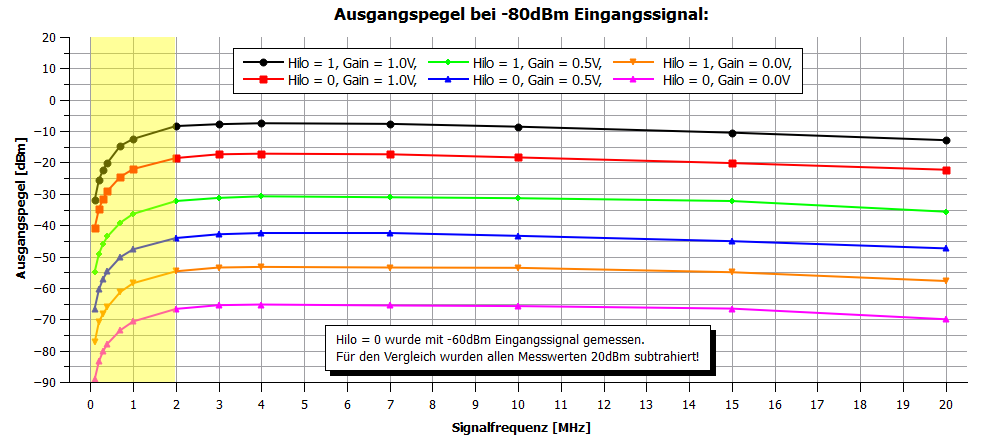
\includegraphics[width=1\textwidth]{data/images/ganzes_system_vorganger}
    \caption{Verstärkung des AD8331 und ISL55210. Gemessen im Vorgängerprojekt\cite{SDRprev}.}
    \label{fig:ganzes_system_vorganger}
\end{center}
\end{figure}

Bei dieser Kurve gibt es einen Unerwarteten Abfall bei 2 MHz abwärts, was in der Vorgängerarbeit auf das aktive Impedanzmatching geschoben wurde. Dieses Verhalten konnte in den gemachten Messungen nicht nachvollzogen werden. Im Gegenteil, es wird ein starker Anstieg gemessen in diesem Bereich.

Ein dritter Punkt ist, dass der Verstärker einen unerwarteten Abfall hat je höher die Frequenz ist. Laut Datasheet sollte der Verstärker locker bis 100MHz um 28 dB verstärken. Die Kurve müsste relativ gerade ausfallen. Erst war der Gedanke da, dass es nur ein Fehle rin diesem Projekt ist. Wie sich aber zeigt bestand dieses Verhalten schon im Vorgängerprojekt, wurde jedoch nicht explizit bemerkt oder wenigstens erwähnt.

Erst viel zu spät wurde dann wenigstens noch bemerkt dass der AD8331 vollig falsch belastet wurde, da nach der Einzelmessung des AD8331 die Widerstände R7 und R8 auf 0 $\Omega$ belassen wurden statt diese korrekterweise auf 250 $\Omega$ anzupassen. Dies ist wichtg damit der AD8331 keine zu grosse last hat welche er nicht zu treiben vermag und dann komische Dinge tut.

Nach dem Wechsel sahen die Resultate waren die Resultate ganz akzeptabel!

\begin{figure}[H]
\begin{center}
    \includegraphics[width=1\textwidth]{data/images/messungen/vga_lna_2016-01-18_50dBm_10dB_HI_rez}
    \caption{Verstärkung des AD8331 und ISL55210 50 MHz Sweep bei 10 verschiedenen Verstärkungen.}
    \label{fig:T_fixed_ISL55210}
\end{center}
\end{figure}

In dieser Grafik kann ohne weiteres erkannt werden, dass im ISL55210 ungewollt $1.5 \frac{dB}{dec}$ verliert. Dieser Effekt ist gar nicht toll. zwar gehen bei 30 MHz nur 2.5 dB verloren, jedoch ist die Tatsache dass der Effekt existiert beunruhigend, da anscheinend etwas noch immer nicht korrekt ist. Dies kann natürlich noch immer an der Terminierung liegen.

\begin{figure}[H]
\begin{center}
    \includegraphics[width=1\textwidth]{data/images/messungen/vga_lna_2016-01-18_50dBm_10dB_HI_rez_mean}
    \caption{Verstärkung des AD8331 und ISL55210 gemittelt über einen 50 MHz Sweep. Ist und Soll gegenübergestellt. Zudem die Differenz zu jedem Wert.}
    \label{fig:T_fixed_mean_ISL55210}
\end{center}
\end{figure}

Wie gut erkannt werden kann ist der Fehler der am ISL55210 entsteht grösser als derjenige, der am AD8331 entsteht. Jedoch ist der Fehler über dem ISL55210 mit weniger als 1.5 dB immernoch sehr klein. Die Abweichung zum erwarteten Wert entsteht wohl dadurch, dass zum einen die Terminierung mit 270 $\Omega$ zwischen AD8331 und ISL55210 zu hoch gewählt ist (250 $\Omega$ wären korrekt) und der Messadapter mit 250 $\Omega$, welche für den AD8331 benötigt wurden, ebenfalls einen zu hohen Widerstand hat (200 $\Omega$ wären korrekt). Wahrscheinlich der wichtigste Punkt ist aber dass die Feedbackwiderstände am AD8331 nicht eine so hohe Genauigkeit haben, dass die Effektive Verstärkung variiert.

\clearpage

\section{Resultate}
\label{sec:resultate}
% BOTH

\clearpage
\bibliography{main,example,IEEEabrv}

\end{document}

